\section{January 2022}

\subsection*{Classical Mechanics}
\addcontentsline{toc}{subsection}{Classical Mechanics}

\prob{1.1}{

With the Lagrangian $\mathcal{L} = T - V$, the Euler-Lagrange equations of motion are given by
\begin{align*}
    \dv{t} \Big( \pdv{\mathcal{L}}{\dot{q}_i} \Big) - \pdv{\mathcal{L}}{q_i} = 0
.\end{align*}
We can modify these equations by introducing a function $\mathcal{F}(\dot{q}_i)$ that depends on the velocities only, writing expanded equations as follows:
\begin{align*}
    \dv{t} \Big( \pdv{\mathcal{L}}{\dot{q}_i} \Big) - \pdv{\mathcal{L}}{q_i} + \pdv{\mathcal{F}}{\dot{q}_i} = 0
\end{align*}
Let the Lagrangian for a system with one degree of freedom, $x$, be given by
\begin{align*}
    \mathcal{L} = \frac{m}{2} \dot{x}^2 - \frac{k}{2} x^2
\end{align*}
and
\begin{align*}
    \mathcal{F} = \eta \dot{x}^2
,\end{align*}
where $\eta > 0$.

\begin{parts}
    \item Write down the expanded equation of motion defined above.

    \item What system is described by this equation of motion?

    \item Find an ansatz for the general solution (you may write $x(t)$ as a potentially complex-valued function which simplifies the math).

    \item Show that your ansatz solves the expanded equation of motion.

    \item Discuss the three difference cases for the solution, depending on $k$, $m$, and $\eta$.
\end{parts}

}

\sol{

(a) The expanded equation of motion is given as follows:
\begin{align}
    \eqbox{ m \ddot{x} + 2 \eta \dot{x} + k x = 0 }
.\end{align}

(b) The system described above is a simple, damped harmonic oscillator (a mass on a spring with non-negligible drag from the fluid it is placed in).

(c) We can write a solution ansatz as $x(t) = A e^{i \omega t}$.
Note that the physical solution is the real part of this, where $A$ is complex and therefore encodes a phase as well.

(d) Plugging in our ansatz, we have
\begin{align}
    A \Big( -m \omega^2 + 2 i \eta \omega - k \Big) e^{i \omega t} = 0 \Rightarrow \eqbox{ \omega_{\pm} = i \beta \pm \sqrt{\omega_0^2 - \beta^2} }
,\end{align}
where we have defined $\omega_0 = \sqrt{k/m}$ and $\beta = \eta / m$.

(e) There are three situations, governed by the sign of the radicand.
First, if $\omega_0 > \beta$, then we have an underdamped situation
\begin{align}
    \eqbox{ x(t) = A e^{-\beta t} \cos(\Omega t + \gamma) }
,\end{align}
where $\Omega = \sqrt{\omega_0^2 - \beta^2}$ and $A,\gamma$ are constants determined by initial conditions.
Next, if $\omega_0 = \beta$, then we have perfectly damped motion
\begin{align}
    \eqbox{ x(t) = e^{-\beta t} ( A + B t ) }
,\end{align}
where $A,B$ are constants determined by initial conditions.
Note that in this case, the radicand is zero and $\omega_+ = \omega_-$.
It turns out that $t e^{-\beta t}$ is a linearly independent solution from the purely damped exponential, which can be checked \textit{a posteriori}, or derived by factoring the second order differential operator as in the difference of squares.
Lastly, we have the overdamped situation, where
\begin{align}
    \eqbox{ x(t) = e^{-\beta t} \Big[ A e^{-\kappa t} + B e^{\kappa t} \Big] }
,\end{align}
where again $A,B$ are determined by initial conditions and $\kappa = \sqrt{\beta^2 - \omega_0^2}$.

}


\prob{1.2}{

A mathematical pendulum of length $l$ and mass $m$ is in a gravitational field with normal acceleration $g$ along the $-y$ axis.
The suspension point $O$ of the pendulum is driven by a motor along $x$ in such a way that the suspension point oscillates as shown in the Figure.

\begin{parts}
    \item Write down the Lagrangian of the system in terms of time-dependent coordinate of the suspension point $x(t)$ and the angle $\varphi(t)$.

    \item Write down a dynamic equation for $\varphi(t)$ and solve it for small-amplitude oscillations of $\varphi(t) \ll 1$ caused by the oscillating suspension point with $x(t) = x_0 \sin{\omega t}$ and $x_0 \ll l$.
\end{parts}

\begin{center}
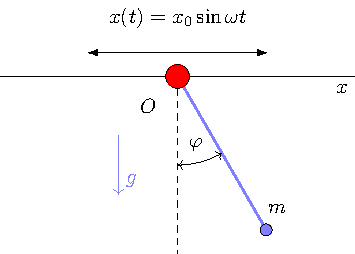
\includegraphics{January2022/1-2.pdf}
\end{center}

}

\sol{

(a) The coordinates of the mass are given by
\begin{align}
    x = x_s + l \sin{\varphi}, \quad y = - l \cos{\varphi}
,\end{align}
where $x_{s}$ is the horizontal position of the suspension point,
so
\begin{align}
    \dot{x} = \dot{x}_s + l \dot{\varphi} \cos{\varphi}, \quad \dot{y} = l \dot{\varphi} \sin{\varphi}
.\end{align}
From this, we see that the Lagrangian
\begin{align}
    L &= \frac{m}{2} \Big[ (\dot{x}_{s} + l \dot{\varphi} \cos{\varphi})^2 + l^2 \dot{\varphi}^2 \sin^2{\varphi} \Big] + m g l \cos{\varphi} \nonumber \\
    &= \eqbox{ \frac{m}{2} \Big[ l^2 \dot{\varphi}^2 + 2 l \dot{x}_{s} \dot{\varphi} \cos{\varphi} + \dot{x}_{s}^2 \Big] + m g l \cos{\varphi} }
.\end{align}


(b) We can write down the equation of motion as follows:
\begin{align}
    m l^2 \ddot{\varphi} + ml( \ddot{x}_{s} \cos{\varphi} - \dot{x}_{s} \dot{\varphi} \sin{\varphi} ) + m g l \sin{\varphi} = 0
.\end{align}
If we introduce the prescribed motion of the suspension point and assume small oscillations
\begin{align}
    \eqbox{ \ddot{\varphi} + \Big( \frac{g}{l} - \frac{x_0 \omega}{l} \cos{\omega t} \Big) \varphi  = \frac{x_0 \omega^2}{l} \sin{\omega t} }
.\end{align}
If we assume that $x_0 \omega \ll g$, then the equation of motion looks like a driven oscillator with natural frequency $\omega_0 = \sqrt{g / l}$.
Thus,
\begin{align}
    \eqbox{ \varphi(t) = A \cos(\omega_0 t + \gamma) + \frac{x_0/l}{(\omega_0 / \omega)^2 - 1} \sin{\omega t} }
,\end{align}
where $A, \gamma$ are constants to be determined by initial conditions.

}


\prob{1.3}{

The Lagrangian $L(\vb*{r}_i,\dot{\vb*{r}}_i)$ is invariant under rotations about an axis whose direction is specified by the unit vector $\vu*{n}$.
Here $\vb*{r}_i$ and $\dot{\vb*{r}}_i$ are the positions and velocities of particles $i = 1,\cdots,N$.
Knowing that under an infinitesimal rotation by an angle $\eta$ about $\vu*{n}$ a generic vector $\vb*{v}$ changes as
\begin{align*}
    \vb*{v} \rightarrow \vb*{v}' = \vb*{v} + \eta \, \vu*{n} \times \vb*{v}
,\end{align*}
show that the projection of the total angular momentum along $\vu*{n}$ is conserved.

}

\sol{

Under the same rotation, the angular momentum
\begin{align}
    \vb*{L}' &= \vb*{r}' \cross \vb*{p}' = ( \vb*{r} + \eta \vu*{n} \cross \vb*{r} ) \cross (\vb*{p} + \eta \vu*{n} \cross \vb*{p}) = \vb*{L} + \eta [ \vb*{r} \cross (\vu*{n} \cross \vb*{p}) - \vb*{p} \cross ( \vu*{n} \cross \vb*{r} ) ] \nonumber \\
    &= \vb*{L} + \eta [ \vb*{r} ( \vu*{n} \cdot \vb*{p} ) - \vb*{p} ( \vu*{n} \cdot \vb*{r} ) ] = \vb*{L} + \eta \vu*{n} \cross \vb*{L}
.\end{align}
Note that we have neglected the terms of $\mathcal{O}(\eta^2)$.
From this form, it is obvious that $\vb*{L}' \cdot \vu*{n} = \vb*{L} \cdot \vu*{n}$.

}


\prob{1.4}{

In a particle accelerator the momentum compaction factor $\alpha$ is a dimensionless number equal to the ratio of the relative change of the path length and the relative change of the momentum
\begin{align*}
    \alpha = \frac{\delta L}{L} \Big/ \frac{\delta p}{p} = \frac{p}{L} \dv{L}{p}
\end{align*}
Consider a satellite in a circular orbit.
What is the momentum compaction factor?

You may assume that the change of momentum is small and slow enough that the orbit is always circular.

}

\sol{

For circular paths, the path length is just the circumference of a circle with radius $R$: $L = 2 \pi R$.
Additionally, since the path is circular, the centrifugal and gravitational forces are always in equilibrium, allowing us to write
\begin{align}
    \frac{G M m}{R^2} = \frac{m v^2}{R} = \frac{p^2}{m R} \Rightarrow L = \frac{2 \pi G M m^2}{p^2}
.\end{align}
Thus
\begin{align}
    \eqbox{ \alpha = -\frac{p}{L} \frac{4 \pi G M m^2}{p^3} = -2 }
.\end{align}

}


\prob{2.1}{

In a simple Atwood machine, two masses are suspended, under constant gravity, from the ends of a flexible, massless, inextensible rope that passes over an inertialessly rotating pulley.
Here, the two masses $m_1$ and $m_2$, the rope is of length $l$, and the constant gravitational acceleration $g$ is downward.

\begin{center}
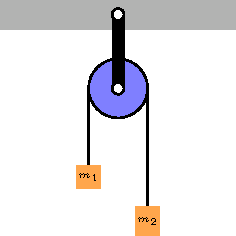
\includegraphics{January2022/2-1.pdf}
\end{center}

Suppose that the second mass is replaced by a live monkey of equal mass that climbs up the rope at speed $v(t)$ relative to the rope.
Treating the monkey's motion as a (time-dependent) constraint in the Lagrangian formalism, answer the following questions:
\begin{parts}
    \item Find the acceleration of the mass, $m_1$, if the monkey climbs up the rope with constant speed $v$.

    \item Find the acceleration of the mass $m_1$, if the monkey climbs up the rope with constant acceleration $\dot{v}(t) = a$.
\end{parts}

}

\sol{

(a) Let's solve this problem in the Lagrangian fomalism.
We have two constraints.
First, the length of the rope is constant $x_1 + x_2 = L$, where $x_1$ and $x_2$ are the heights of the ends of the rope from some reference.
Second, we have $x_2 + \Delta x = x$, where $\Delta x$ is the height of the monkey relative to the end of the rope and $x$ is its height relative to the absolute reference point.
We then have as our Lagrangian
\begin{align}
    L &= \frac{m_1 \dot{x}_{1}^2}{2} + \frac{m_2 \dot{x}^2}{2} - m_1 g x_1 - m_2 g x \nonumber \\
    &= \frac{m_1 \dot{x}_{1}^2}{2} + \frac{m_2 ( v - \dot{x}_{1} )^2}{2} - m_1 g x_1 - m_2 g L + m_2 g x_1 - m_2 g \Delta x
.\end{align}
The equation of motion for $x_1$ is
\begin{align}
    ( m_1 + m_2 ) \ddot{x}_{1} + ( m_1 - m_2 ) g = m_2 \dot{v} \Rightarrow \ddot{x}_1 = \frac{m_2 \dot{v} + (m_2 - m_1) g}{m_1 + m_2}
.\end{align}

If we have constant $v$, then
\begin{align}
    \eqbox{ \ddot{x}_1 = \frac{m_2 - m_1}{m_1 + m_2} g }
.\end{align}


(b) If we instead have $\dot{v} = a$, where $a$ is constant,
\begin{align}
    \eqbox{ \ddot{x}_1 = \frac{m_2 a + (m_2 - m_1) g}{m_1 + m_2} }
.\end{align}

}

\subsection*{Electricity \& Magnetism}
\addcontentsline{toc}{subsection}{Electricity \& Magnetism}

\prob{2.2}{

Consider the region between two concentric spherical surfaces of radii $a$ and $b$.
On the inner boundary ($r = a$) of this region, the potential is constant,
\begin{align*}
    \phi(a,\theta) = 2 V_0
.\end{align*}
On the outer boundary ($r = b$) of this region, the potential is given by
\begin{align*}
    \phi(b,\theta) = V_0 \cos{\theta}
.\end{align*}

\begin{parts}
    \item Find the potential in the region $a \leq r \leq b$.

    \item Now suppose that the region between two concentric spherical surfaces is filled with the inhomogeneous charge density $\rho(\vb*{r}) = \lambda / r$, where $\lambda$ is a constant and $r$ is the distance to the center of the spheres.
    The potentials on the spherical surfaces are kept the same as in part (a).

    Find the solution of the Poisson equation in the region $a \leq r \leq b$.

    (Note: The inner and outer surfaces have surface charges that can create non-spherically symmetric potentials.)
\end{parts}

}

\sol{

(a) The relevant equation for this problem is Laplace's equation.
Since our geometry is spherical with azimuthal symmetry, we can immediately write
\begin{align}
    \Phi(\vec{r}) = \sum_{l} P_{l}(\cos{\theta}) \begin{cases}
        A_l r^l & r < a \\
        B_l r^l + C_l/r^{l+1} & a < r < b \\
        D_l / r^{l+1} & r > b
    \end{cases}
.\end{align}
We have two boundary conditions are each interface:
\begin{align}
    &(i) ~ \Phi(a) = 2 V_0 \\
    &(ii) ~ \Phi(a^{-}) = \Phi(a^{+}) \\
    &(iii) ~ \Phi(b) = V_0 \cos{\theta} \\
    &(iv) ~ \Phi(b^{-}) = \Phi(b^{+})
.\end{align}
The first gives us that
\begin{gather}
    \sum_l A_l a^l P_l(\cos{\theta}) = 2 V_0 \nonumber \\
    \sum_l A_l a^{l} \underbrace{ \int_{-1}^{1} \dd{(\cos{\theta})} P_{l}(\cos{\theta}) P_m(\cos{\theta}) }_{2/(2m + 1) \delta_{lm}} = 2 V_0 \int_{-1}^{1} \dd{(\cos{\theta})} P_0(\cos{\theta}) P_{m}(\cos{\theta}) \nonumber \\
    \frac{2}{2 m + 1} A_m a^m = 4 V_0 \delta_{m 0} \Rightarrow A_l = 2 V_0 \delta_{l 0}
.\end{gather}
The third condition by a similar argument and using that $P_1(\cos{\theta}) = \cos{\theta}$ yields $D_l = V_0 b^2 \delta_{l 1}$.
Next, we apply our continuity conditions:
\begin{align}
    A_l a^{2 l + 1} = B_l a^{2 l + 1} + C_l \\
    B_l b^{2 l + 1} + C_l = D_l
,\end{align}
which give
\begin{align}
    B_l &= \frac{D_l - A_l a^{2l + 1}}{b^{2l+1} - a^{2 l + 1}} = V_0 \Bigg[ \frac{b^2}{b^{3} - a^{3}} \delta_{l1} - \frac{2 a}{b - a} \delta_{l 0} \Bigg] \\
    C_l &= - \frac{a^{2l + 1}}{b^{2 l + 1} - a^{2 l + 1}} D_l + \frac{a^{2l+1}b^{2l+1}}{b^{2l+1} - a^{2l+1}} A_l = V_0 \Bigg[ \frac{2 a b}{b - a} \delta_{l 0} - \frac{a^3 b^2}{b^3 - a^3} \delta_{l1} \Bigg]
.\end{align}
Thus,
\begin{align}
\eqbox{
    \Phi(r,\theta) = V_0 \begin{cases}
        2 & r < a \\
        \frac{2}{b/a - 1} \Big( \frac{b}{r} - 1 \Big) + \Big( \frac{1}{1 - (a/b)^3} \frac{r}{b} - \frac{1}{(b/a)^3 - 1} \frac{b^2}{r^2} \Big) \cos{\theta} & a < r < b \\
        \frac{b^2}{r^2} \cos{\theta} & r > b
    \end{cases}
}
\end{align}


(b) We can do as requested by superimposing the solution from above with that of two grounded conductors with the specified volume charge density between the spheres.
Since the additional problem is spherically symmetric, we can use Gauss' law:
\begin{align}
    \oint \vb*{E} \cdot \dd{\vb*{A}} = \frac{Q}{\epsilon_0} \Rightarrow E(r) = \frac{Q_{a} + Q(r)}{4 \pi \epsilon_0} \frac{1}{r^2}
,\end{align}
where $Q(r)$ is the charge enclosed by our Gaussian surface, which we choose to be a sphere of radius $r$, and $Q_{a}$ is the charge on the inner sphere.
We can compute the charge
\begin{align}
    Q(r) = 4 \pi \lambda \int_{a}^{r} r \dd{r} = 2 \pi \lambda ( r^2 - a^2 )
.\end{align}
The electric field is then
\begin{align}
    \vb*{E} = \frac{Q_a + 2 \pi \lambda (r^2 - a^2)}{4 \pi \epsilon_0 r^2}
,\end{align}
and the potential is just
\begin{align}
    \Phi(r) = \frac{1}{4 \pi \epsilon_0} \int_{r}^{b} \frac{Q_{a} + 2 \pi \lambda (r^2 - a^2)}{r^2} \dd{r} = \frac{1}{4 \pi \epsilon_0} \Bigg[ (Q_{a} - 2 \pi \lambda a^2) \Big( \frac{1}{r} - \frac{1}{b} \Big) + 2 \pi \lambda ( b - r ) \Bigg]
.\end{align}
The form of the potential above gurantees that the outer sphere is grounded.
We now solve for $Q_{a}$ such that the inner sphere is also grounded as needed:
\begin{align}
    (Q_{a} - 2 \pi \lambda a^2) \Big( \frac{1}{a} - \frac{1}{b} \Big) + 2 \pi \lambda ( b - a ) = 0 \Rightarrow Q_{a} = -2 \pi \lambda a ( b - a )
.\end{align}
Plugging this in, we find
\begin{align}
    \Phi(r) = 2 \pi \lambda \Bigg[ (b - r) - a \Big( \frac{b}{r} - 1 \Big) \Bigg]
\end{align}
as the potential between the spheres, and using the same line integration, we see that the potential is zero for this setup when $r < a$ and $r > b$.

Now that we have our results, the composite potential with the charge density between the spheres and the potential $2 V_0$ and $V_0 \cos{\theta}$ on the inner and outer spheres is
\begin{align}
    \eqbox{ \Phi(r,\theta) = \begin{cases}
        2 V_0 & r < a \\
        \frac{2 V_0}{b/a - 1} \Big( \frac{b}{r} - 1 \Big) + V_0 \Big( \frac{1}{1 - (a/b)^3} \frac{r}{b} - \frac{1}{(b/a)^3 - 1} \frac{b^2}{r^2} \Big) \cos{\theta} + 2 \pi \lambda \Big[ (b - r) - a \Big( \frac{b}{r} - 1 \Big) \Big] & a < r < b \\
        \frac{V_0 b^2}{r^2} \cos{\theta} & r > b
    \end{cases}
}
.\end{align}


}


\prob{2.3}{

Consider a straight wave-guide of arbitrary but constant cross-section.
The walls inside the wave-guide are ideal conductors (infinite conductivity) and the interior of the wave-guide is a vacuum.
The lowest cutoff frequency is $\omega_0$ and the next higher one is $\omega_1$.
The wave-guide is excited at the frequency $\omega$ such that $\omega_0 < \omega < \omega_1$.

For the waves that are propagating down the wave-guide, what are the phase velocity and the group velocity?

}

\sol{

Recall that the relevant equation for wave-guides, regardless of the mode, is 
\begin{align}
    (\grad_T^2 + \gamma^2) \psi = 0
,\end{align}
where $\psi = E_z,B_z$ and $\gamma = \mu \epsilon \omega^2 - k^2$.
The allowed values of $\gamma$ denoted by $\gamma_n$ are determined by boundary conditions (i.e. the geometry of the wave-guide).
We can define the cutoff frequency for the $n^{\rm th}$ mode via
\begin{align}
    \gamma_n^2 = \mu \epsilon \omega_n^2
,\end{align}
which allows us to express
\begin{align}
    k = \sqrt{\mu \epsilon} \sqrt{\omega^2 - \omega_n^2} = \frac{1}{c} \sqrt{\omega^2 - \omega_{n}^2}
.\end{align}
The phase velocity is defined by
\begin{align}
    \eqbox{ v_p = \frac{\omega}{k} = \Big( \frac{k}{\omega} \Big)^{-1} = \frac{c}{\sqrt{1 - (\omega_n / \omega)^2}} }
,\end{align}
and the group velocity is
\begin{align}
    \eqbox{ v_g = \dv{\omega}{k} = \Big( \dv{k}{\omega} \Big)^{-1} = c \sqrt{1 - (\omega_n / \omega)^2} }
.\end{align}
Note that these are phase and group velocities for the $n^{\rm th}$ mode.

}


\prob{2.4}{

A charge is uniformly distributed on the surface of a solid sphere, which rotates with a fixed angular velocity about an axis through its center.
The sphere is in a uniform and constant magnetic field with a nonzero angle relative to the sphere's axis of rotation.
Without doing any detailed calculations, describe the motion of the sphere, justifying your reasoning.
What happens to the sphere's axis of rotation?

}

\sol{

Let us orient our coordinate system so that the $z$-axis aligns with the angular velocity of the rotation.
Similarly, let's orient the magnetic field at an angle $\theta$ relative to the $z$-axis fixed in the $zy$-plane.
The rotating charges constitute a surface current $\vb*{K}$, whose direction is given by $\vu*{\phi}$.
The force on the sphere is proportional to the vector product $\int \dd[3]{\vb*{r}} \vb*{K} \cross \vb*{B}$.
Since the field is constant and we are in the realm of magnetostatics, there is no net force on the sphere.
Another consideration, however is the torque on the sphere, which is proportional to $\int \dd[3]{\vb*{r}} \vb*{r} \cross ( \vb*{K} \cross \vb*{B} )$, which is nonzero unless $\vb*{B}$ and $\vb*{K}$ are (anti-)parallel.
This torque will cause the axis of rotation to precess around the magnetic field.

}


\prob{3.1}{

A conducting surface held at zero potential consists of a plane with a hemispherical bump of radius $R$ (see the figure below).
A charge $q$ sits a distance $r > R$ above the center of the hemispherical bump.

\begin{center}
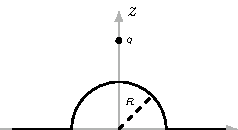
\includegraphics{January2022/3-1.pdf}
\end{center}

Calculate the force on the charge.

\textbf{Hint}: Use image charges.
Note that you may need more than one image charge; in fact, as many as three.
You should verify that your image solution satisfies the correct boundary conditions.

}

\sol{

We know how to place two charges already.
First we have $q_1$ as if the setup was only the plane: $q_1 = -q$ at $z = -r$.
Next, we have $q_2$ as if the setup was only the sphere: $q_2 = -q(R/r)$ at $z = R^2 / r$.
Notice though that we are not done.
The charges $q$ and $q_1$ cancel on the plane, leaving the contribution of $q_2$.
Meanwhile, the charges $q$ and $q_2$ cancel on the hump, leaving the contribution of $q_1$.
We should place a third charge which simultaneously cancels both of these unbalanced contributions.
After some inspection, we can place a charge $q_3 = (R/r) q$ at $z = -R^2/r$, which cancels both happily on the needed surfaces.
From this, the force on the charge $q$ is
\begin{align}
    \vec{F} = \frac{q^2}{4 \pi \epsilon_0} \Bigg[ -\frac{R/r}{(r - R^2 / r)^2} + \frac{R/r}{(r + R^2/r)^2} - \frac{1}{(2r)^2} \Bigg] \vu*{z} = -\frac{q^2}{4 \pi \epsilon_0} \Bigg[ \frac{2 r^3 R^3}{(r^4 - R^4)^4} + \frac{1}{4 r^4} \Bigg] \vu*{z}
\end{align}

}

\prob{3.2}{

A particle with charge $q$ and mass $m$ moves in a parabolic potential $U(x,y,z) = k(x^2 + y^2 + z^2)/2$, and a constant magnetic field $B$ is applied along the $z$-axis.

\begin{parts}
    \item Write down the equations of motion.

    \item How does the frequency of this 3D charged oscillator change owing to the presence of this constant magnetic field?

    \item Describe the trajectories of the oscillator corresponding to its different eigenfrequencies in the magnetic field.
\end{parts}

}

\sol{

The force acting on the charge is given as
\begin{align}
    m \ddot{\vb*{r}} = q \dot{\vb*{r}} \cross B \vu*{z} - k (x \vu*{x} + y \vu*{y} + z \vu*{z})
.\end{align}
In component form, we have
\begin{align}
\eqbox{
\begin{aligned} 
    \ddot{x} &= \frac{q B_z}{m} \dot{y} - \frac{k}{m} x \\
    \ddot{y} &= - \frac{q B_z}{m} \dot{x} - \frac{k}{m} y \\
    \ddot{z} &= -\frac{k}{m} z
.\end{aligned}
}
\end{align}


(b) The oscillation in the $z$ direction is unchanged as a result of the existence of the magnetic field.
If we insert $x = A e^{i \omega t}$ and $y = B e^{i \omega t}$, then
\begin{align}
    \begin{pmatrix}
        \omega^2 - \omega_0^2 & i \omega \omega_c \\
        -i \omega \omega_c & \omega^2 - \omega_0^2
    \end{pmatrix}
    \begin{pmatrix}
    A \\ B
    \end{pmatrix}
    = 0
,\end{align}
where $\omega_0 = \sqrt{k/m}$ and $\omega_c = q B_z / m$.
This is solved by requiring the matrix to have zero determinant, yielding
\begin{align}
    \eqbox{ \omega_{\pm}^2 = \omega_0^2 + \frac{\omega_{c}^2}{2} \pm \omega_c \sqrt{\omega_0^2 + \frac{\omega_{c}^2}{4}} }
.\end{align}
The positive branch corresponds to strictly oscillatory motion.
If $\omega_{c} \sqrt{\omega_0^2 + (\omega_{c}/2)^2} > \omega_0^2 + \omega_{c}^2 / 2$, then the negative branch corresponds to damped motion, which dies out over time and leaves only the first oscillation mode.
If they are equal, then the 

}


\prob{3.3}{

Until 2019, the definition of the Ampere was as follows:
\textit{The ampere is that constant
current which, if maintained in two straight parallel conductors of infinite length,
of negligible circular cross-section, and placed 1 meter apart in vacuum, would
produce between these conductors a force equal to $2 \times 10^{-7}$ newton per meter of
length.}

\begin{center}
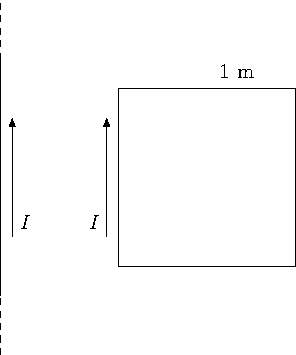
\includegraphics{January2022/3-3.pdf}
\end{center}

Obviously, this was a very impractical definition (``infinitely long, zero cross section wires'').
However, one \textit{can} approximate the implied measurement in the following way:
Consider a quadratic loop of wire, with a side length of $1~{\rm m}$ distance (and, yes, the wires are nearly infinitely thin yet totally rigid).

If we run a current $I$ of $1~{\rm Ampere}$ through both the square and the infinite wire, what will be the force that each conductor exerts on the other?
You may use symmetry arguments as much as possible to simplify the calculation, keeping in mind that we are only interested in the \textbf{net} force.

}

\sol{

The force on a current density is given generically by
\begin{align}
    \vec{F} = \int \dd[3]{\vec{x}} \vec{J}(\vec{x}) \cross \vec{B}(\vec{x})
,\end{align}
which reduces to
\begin{align}
    \vec{F} = I \int \dd{\vec{l}} \cross \vec{B}(\vec{x})
.\end{align}
Before doing any integration, we should determine the magnetic field from the straight wire using Ampere's law:
\begin{align}
    \oint \vec{B} \cdot \dd{\vec{l}} = B_{\phi} (2 \pi r) = \mu_0 I \Rightarrow \vec{B} = \frac{\mu_0 I}{2 \pi r} \vu*{\phi}
,\end{align}
where the direction of $\vu*{\phi}$ is determined by the right-hand rule.
For the purposes of calculation, let's set our origin at the lower left corner of the square with the $x$ axis pointing to the right and $y$ pointing up.
Thus, at the square loop, the magnetic field points in the $-z$ direction.
Quantitatively, we have
\begin{align}
    \vec{F} &= \frac{\mu_0 I^2}{2 \pi} \Bigg\{ \int_{0}^{l} \frac{\dd{y} \vu*{y} \cross (-\vu*{z})}{L} + \int_{0}^{l} \frac{\dd{x} \vu*{x} \cross (-\vu*{z})}{L + x} + \int_{0}^{l} \frac{-\dd{y} \vu*{y} \cross (-\vu*{z})}{L + l} + \int_{0}^{l} \frac{-\dd{x} \vu*{x} \cross (-\vu*{z})}{L + x} \Bigg\} \nonumber \\
            &= \frac{\mu_0 I^2}{2 \pi} \Bigg\{ -\vu*{x} \frac{l}{L} + \vu*{x} \frac{l}{L + l} \Bigg\} = \eqbox{ -\frac{\mu_0 I^2 l^2}{2 \pi L(L + l)} \vu*{x} }
\end{align}


}


\subsection*{Quantum Mechanics}
\addcontentsline{toc}{subsection}{Quantum Mechanics}

\prob{3.4}{

Consider a spinless particle with mass $m$ in the three-dimensional potential $V(r) = Cr^2$ with $C > 0$.

\begin{parts}
    \item What are the energy eigenvalues?
    What are the degeneracies of the three lowest energy eigenvalues?

    \item Suppose that five identical noninteracting particles with mass $m$ move in this potential.
    What is the ground state energy of this system if the particles have (i) spin-1/2, (ii) spin-1?
\end{parts}

}

\sol{

(a) Observe that the potential is that of a harmonic oscillator with frequency $\omega = \sqrt{2 C / m}$.
Knowing this, we can immediately write
\begin{align}
    \eqbox{ E_{n_x,n_y,n_z} = \hbar \omega ( n_x + n_y + n_z + 3/2 ) = \hbar \omega ( n + 3/2 ) = E_n }
.\end{align}
The degeneracies of the three lowest eigenvalues are as follows:
\begin{align}
    \eqbox{ E_0: ~ g_0 = 1, \quad E_1:~g_1 = 3, \quad E_2: ~ g_2 = 6 }
.\end{align}


(b) If we have five non-interacting spin-1/2 particles in this potential, the ground state energy
\begin{align}
    \eqbox{ E = 2 E_0 + 3 E_1 = \frac{21}{2} \hbar \omega }
,\end{align}
while if we have five non-interacting spin-1 particles the ground state energy
\begin{align}
    \eqbox{ E = 5 E_0 = \frac{15}{2} \hbar \omega }
.\end{align}
The essential observation is that identical fermions cannot exist in the same state (i.e. the Pauli exclusion principle), while identical bosons can exist in the same state.

}


\prob{4.1}{

The Pauli spin matrices in quantum mechanics are given by
\begin{align*}
    \sigma_1 = \begin{pmatrix}
        0 & 1 \\ 
        1 & 0
    \end{pmatrix}
    , \quad
    \sigma_2 = \begin{pmatrix}
        0 & -i \\ 
        i & 0
    \end{pmatrix}
    , \quad
    \sigma_3 = \begin{pmatrix}
        1 & 0 \\
        0 & -1
    \end{pmatrix}
.\end{align*}
By definition,
\begin{align*}
    e^{\alpha \sigma_1} = \sum_{n=0}^{\infty} \frac{\alpha^n}{n!} \sigma_1^n
.\end{align*}

\begin{parts}
    \item Calculate $e^{\alpha \sigma_1}$ as an explicit 2 by 2 matrix.

    \item Find eigenvalues and normalized eigenvectors of $e^{\alpha \sigma_1}$.
\end{parts}

}

\sol{

(a) Observe that $\sigma_1^2 = 1$, so
\begin{align}
\eqbox{
\begin{aligned}
    e^{\alpha \sigma_1} &= \sum_{n = 0}^{\infty} \frac{\alpha^n}{n!} \sigma_1^n = \sum_{n=0}^{\infty} \frac{\alpha^{2n}}{(2n)!} \sigma_1^{2n} + \sum_{n=0}^{\infty} \frac{\alpha^{2n+1}}{(2n+1)!} \sigma_1^{2n+1} \\
                        &= \cosh{\alpha} + \sigma_1 \sinh{\alpha} 
    = \begin{pmatrix}
        \cosh{\alpha} & \sinh{\alpha} \\
        \sinh{\alpha} & \cosh{\alpha}
    \end{pmatrix}
\end{aligned}
}
\end{align}


(b) Recall the eigenstates of $\sigma_1$ are
\begin{align}
    \ket{\pm}_x = \frac{1}{\sqrt{2}} \begin{pmatrix}
        1 \\ \pm 1
    \end{pmatrix}
\end{align}
with corresponding eigenvalues $\pm 1$.
Observe that
\begin{align}
    \eqbox{ e^{\alpha \sigma_1} \ket{\pm}_x = ( \cosh{\alpha} \pm \sinh{\alpha} ) \ket{\pm}_x = e^{\pm \alpha} \ket{\pm}_x }
\end{align}

}


\prob{4.2}{

At time $t = 0$ a particle in the potential $V(x) = m \omega^2 x^2 / 2$ is described by the wavefunction
\begin{align*}
    \psi(x,0) = A \sum_n (1/\sqrt{2})^n \psi_n(x)
,\end{align*}
where $\psi_n(x)$ are the orthonormal eigenfunctions of the energy with eigenvalues $E_n = (n+1/2)\hbar \omega$.

\begin{parts}
    \item Find the normalization constant $A$.

    \item Write the expression for $\psi(x,t)$ for $t > 0$.

    \item Show that $| \psi(x,t) |^2$ is a periodic function of time and indicate the period $T$.

    \item Find the expectation value of the energy.
\end{parts}

}

\sol{

(a) The normalization can be determined as follows:
\begin{gather}
    \int \dd{x} |\psi(x,0)|^2 = A^2 \sum_{n,m} \Big( \frac{1}{\sqrt{2}} \Big)^{n+m} \underbrace{ \int \dd{x} \psi_n^*(x) \psi_m(x) }_{\delta_{nm}} = A^2 \sum_n \frac{1}{2^n} = 2 A^2 = 1 \nonumber \\
    \Rightarrow \eqbox{ A = \frac{1}{\sqrt{2}} }
.\end{gather}


(b) We can inject time-dependence into the state using the unitary time-evolution operator:
\begin{align}
    \eqbox{ \psi(x,t) = e^{-i H t / \hbar} \psi(x,0) = \sum_n \Big( \frac{1}{\sqrt{2}} \Big)^{n+1} e^{-i (n + 1/2) \omega t} \psi_n(x) }
\end{align}


(c) Observe that
\begin{align}
    |\psi(x,t)|^2 = \sum_{n,m} \Big( \frac{1}{\sqrt{2}} \Big)^{n+m+2} e^{-i(m - n) \omega t} \psi_n^*(x) \psi_m(x)
.\end{align}
Terms with $n = m$ are constant in time, while the interference terms have period
\begin{align}
    T_{nm} = \frac{2\pi}{(n - m) \omega} = \frac{1}{n-m} T \Rightarrow \eqbox{ T = \frac{2 \pi}{\omega} }
.\end{align}
Notice that $T$ is the period of $|\psi(x,t)|^2$ since this is the largest period of the non-constant interference terms.


}


\prob{4.3}{

A particle of mass $m$ is moving along the $x$-axis (in one dimension), where its potential energy is $V(x) = 0$ for all $x \leq 0$ and $V(x) = V_0$ else.
The particle is in an energy eigenstate with eigenvalue $0 < E < V_0$.

Write down the time-independent Schr\"{o}dinger equation and find a solution (determine all constants to within one overall constant).
What is the probability density for the particle to be found at the classically forbidden point $x = x_0 > 0$, expressed as a fraction of the probability density for the particle to be found at $x = 0$?

}

\sol{

The Sch\"{o}dinger equation reads
\begin{align}
    \dv[2]{\psi}{x} - \Big[ v(x) - k^2 \Big] \psi = E \psi 
,\end{align}
where $k^2 = 2 m E / \hbar^2$ and $v(x) = 2 m V_0 / \hbar^2 \Theta(x)$.
In the region $x < 0$, this reduces to a free-particle, while in the region $x > 0$, we have a particle in a classically forbidden region:
\begin{align}
    \psi(x) = \begin{cases}
        A e^{ikx} + B e^{-ikx} & x < 0 \\
        C e^{-\kappa x} & x > 0
    ,\end{cases}
\end{align}
where $\kappa^2 = v_0 - k^2$.
We can determine two of these constants via the initial conditions
\begin{align}
    \psi(0^{-}) = \psi(0^{+}) \Rightarrow A + B = C \\
    \psi'(0^{-}) = \psi'(0^{+}) \Rightarrow ik ( A - B ) = -\kappa C
.\end{align}
Solving this system, we have
\begin{align}
    \eqbox{ \frac{B}{A} = -\frac{\kappa + ik}{\kappa - ik}, \quad \frac{C}{A} = -\frac{2ik}{\kappa - i k} }
.\end{align}
The probability density for the particle to be found at $x_0 > 0$ relative to that at $x = 0$ is
\begin{align}
    \eqbox{ \Bigg| \frac{\psi(x_0)}{\psi(0)} \Bigg|^2 = \Bigg| \frac{C e^{- \kappa x_0}}{C} \Bigg|^2 = e^{-2 \kappa x_0} }
\end{align}

}


\prob{4.4}{

A particle with spin-1/2 is described by a state vector:
\begin{align*}
    \ket{\chi} = \begin{pmatrix}
        \alpha \\ \beta
    \end{pmatrix}
.\end{align*}
Here $\alpha = e^{i \varphi_1} \cos{\theta}$ and $\beta = e^{i \varphi_2} \sin{\theta}$ are complex amplitudes, and $\theta$, $\varphi_1$, and $\varphi_2$ are real parameters.
Calculate the probabilities to measure the spin +1/2 separately along each of the $x$, $y$, and $z$ axes.

}

\sol{

The probabilities are as follows:
\begin{align}
\eqbox{
\begin{aligned}
    P(S_z = \hbar / 2) &= |\ip{+}{\chi}|^2 = |\alpha|^2 = \cos^2{\theta} \\
    P(S_x = \hbar/2) &= |\ip{+_x}{\chi}|^2 = \frac{1}{2} | \alpha + \beta |^2 = \frac{1}{2} \Big( |\alpha|^2 + |\beta|^2 + \alpha^{*} \beta + \alpha \beta^{*} \Big) \nonumber \\
                     &= \frac{1}{2} \Big[ 1 + 2 \Re(\alpha^{*} \beta) \Big] = \frac{1}{2} \Big[ 1 + \sin(2 \theta) \cos(\varphi_1 - \varphi_2) \Big] \\
    P(S_y = \hbar/2) &= |\ip{+_y}{\chi}|^2 = \frac{1}{2} |\alpha + i \beta|^2 = \frac{1}{2} \Big[ 1 - 2 \Im(\alpha^{*} \beta) \Big] \nonumber \\
                     &= \frac{1}{2} \Big[ 1 + \sin(2 \theta) \sin(\varphi_1 - \varphi_2) \Big]
\end{aligned}
}
\end{align}

}
